\section{Experiments}
\label{sec:eval}

%The following experiments are needed for ACL submission:
%\begin{itemize}
%  \item KBC evaluation on standard dataset. This is what we've done
%        now. We need to show that our schema-base approach performs
%		as good as state-of-the-art.
%  \item KBC evaluation on biased dataset. We need to eyeball PATTY
%        relations and select those complex relations. Then we can
%		compare skeleton-based and schema-based approach.
%  \item QA evalution on biased dataset. Based on complex relations,
%        we find factoid questions (and make some simple modifications
%		if needed) from Yahoo! Answers. And we need to find a way
%		to plug our model in some existing QA systems.
%  \item Relation simialrity dataset to show the expressiveness of
%        compact and human-readable representations, instead of
%		massive features or purely data-driven model.
%		We first extract PPDB relation pairs and eyeball selecting
%		good pairs (no same stemmings in PPDB and corresponding
%		relations in PATTY could get enough entity pairs).
%		This time, ``co-occurrence $\geq$ 1'' should be removed,
%		otherwise we couldn't find enough pairs.
%		Baselines could be word-based w2v, or simply counting EP
%		overlap between different PATTY relation instances.
%\end{itemize}
%
%And we have a list of ablation tests:
%\begin{itemize}
%  \item What's the result if we won't add any constraints?
%  \item What's the result if we change a naive labeling function?
%        Maybe version 4, version 1 and naive ``positive ratio +
%		negative ratio'' could be baselines.
%  \item What's are the running times and results when we change a
%        different budget?
%  \item (Optional) compare the results generated from different
%        negative entity pairs. Maybe some generating strategy can
%		show a better difference of results between skeleton-based
%		and schema-based methods.
%\end{itemize}
%

%In this section, we evaluate the schemas learned from input NL relations.
%We first evaluate the performance on the knowledge
%base completion (KBC) task where the relations come from an Open IE system,
%then we compare with state-of-the-art systems on question answering
%task using questions involving complex relations.
%Finally, we show that our schema representation can be used to compute
%similarity between NL relations and achieve comparable results against
%word embedding models.

In this section, we evaluate the performance on the knowledge base
completion task, and compare our results with the state-of-the-art approach.
Then we show examples of detail schemas inferred by our system, and
analyze our result.
%\subsection{Experiment Setup}
%In our experiments, we use PATTY \cite{nakashole2012patty} as the Open IE system.
%PATTY contains more than 200,000 different relations with
%millions of entity pairs extracted from Wikipedia.
%%To evaluate the quality of paraphrasing, we build two relation datasets containing
%%positive and negative $\langle e_1, r, e_2 \rangle$ relation triples, and perform
%%paraphrasing task over Freebase.
%For experiments in this section, we set the following parameters:
%$\tau$ = 3, $\gamma$ = 10\%, and size of the
%priority queue is 1000.
\begin{table}[ht]
	\small
	\centering
	\caption{Statistics of Freebase used in experiments}
	\begin{tabular}{|c|c|c|}
		%\toprule
		\hline
		Dataset				& $FB$			& $FB^-$ 	\\
        \hline
		Ordinary entities	& 50,718,028	& 3,000,000		\\
        \hline
        Mediator entities	& 36,131,437	& 7,301,261		\\
		\hline
		Total entities		& 86,849,465	& 10,301,261	 \\
		\hline
		Distinct relations	& 4,932			& 4,412			\\
        \hline
		Types 				& 2,071			& 2,063			\\
		\hline
		Total facts			& 280,788,583	& 58,224,932	\\
		\hline
	\end{tabular}%
	\label{tab:fb-size}%
\end{table}

\subsection{KBC Evaluation on Complex Relations}
We first evaluate KBC on complex relations to see how much gain a schema-based approach can attain.
In this evaluation, the system takes relation instances as input,
and predict whether a new entity pair belongs to the particular relation or not.
%As our system generated schema distributions,
In our system, the probability of one entity pair belonging to the relation
equals to sum probability of schemas that covered the entity pair.

In our experiments, we use Freebase dump in June 2015~\cite{freebase:datadumps} as the knowledge base
and PATTY \cite{nakashole2012patty} as the Open IE system.
PATTY contains more than 200,000 different relation synsets
with millions of entity pairs extracted from Wikipedia.
Each entity in PATTY is linked to Freebase through the unique Wikipedia page.
We manually inspect top 1,077 distinct PATTY relations containing at least 100 relation instances,
and in total 61 complex relations are selected for this evaluation.
For each relation, we extract up to 500 entity pairs as positive instances.
Then we generate negative instances for testing and validation by
randomly combining subjects and objects among positive instances.
The ratio of instances between positive and negative data is 1 : 10.
We split all instances in each relation into 80\% training and 20\% testing data.
Besides, we take 20\% instances from training data as the validation set,
which is used to tune a cutoff threshold: entity pairs with probability
larger than the threshold are predicted as true (belong to the relation).
We set the following parameters in the experiment:
$\tau$ = 3, $\gamma$ = 10\%, $\alpha$ = 0.0001 and size of the priority queue is 1000.

%\tabref{tab:complex-example} shows some example relations with
%labeled schemas.
%
%\begin{table}[ht]
%\small
%	\centering
%	\caption{Example complex relations and their schemas.}
%	\begin{tabular}{|c|c|}
%		\hline
%		Relation		& Schema	\\
%        \hline
%        \hline
%		be county of	& contained\_by + IsA($x_{subj}$)=us\_county \\
%        \hline
%		be nephew of 	& \pbox{20cm}{parents + siblings + \\ gender($x_{subj}$)=male} \\
%		\hline
%        professor at	& \pbox{20cm}{employment\_history + at\_company \\  + IsA($x_{obj}$)=university} \\
%		\hline
%		\pbox{10cm}{died from \\ heart attack in}	& \pbox{20cm}{place\_of\_death + \\ cause\_of\_death($x_{subj}$)=heart\_disease} \\
%		\hline
%		\pbox{10cm}{play colledge \\ baseketball in} & \pbox{20cm}{athelete\_played + in\_sports\_team +
%				\\ belong\_to\_school + sport($x_2$)=basketball}	\\
%		\hline
%		study art in	& \pbox{20cm}{educated + at\_institution + \\ IsA($x_{subj}$)=visual\_artist}	\\
%		\hline
%		constituency in	& \pbox{20cm}{contained\_by + \\ IsA($x_{obj}$)=gov\_jurisdiction} \\
%		\hline
%		\pbox{10cm}{{\em PER}'s \\ invasion in} & \pbox{20cm}{nationality + envolved\_in\_conflict + \\
%			military\_combatant + IsA($x_{obj}$)=country \\  + IsA($x_{subj}$)=military\_commander} \\
%		\hline
%	\end{tabular}%
%	\label{tab:complex-example}%
%\end{table}

We first compare our approach with a baseline method,
which only takes skeletons as candidates (without searching constraints).
The upper part of \tabref{tab:kbc-complex} shows a clear gap
between schema-based approach and the baseline method. 
We found that skeleton baseline tends to predict more entity pairs,
but it failed to maintain an acceptable precision.
While our schema approach made a good balance between precision and recall,
thus it produced a much better result.




\begin{table}[ht]
	\small
	\centering
	\caption{KBC results on 61 complex relations.}
	\begin{tabular}{|c||c|c|c|c|}
		%\toprule
		\hline
		Dataset					& Approach	& Precision & Recall & F1 \\
        \hline
		\multirow{2}{*}{$FB$}	& Schema	& \textbf{0.619} & 0.497 & \textbf{0.551} \\
		\cline{2-5}
        						& Skeleton	& 0.454 & \textbf{0.533} & 0.490 \\
		\hline
		\multirow{4}{*}{$FB^-$} & Schema		& \textbf{0.596} & 0.504 & \textbf{0.547} \\
		\cline{2-5}
								& Skeleton		& 0.444	& 0.541	& 0.488	\\
		\cline{2-5}
								& SFE-AnyRel	& 0.378	& \textbf{0.574} & 0.456	\\
		\cline{2-5}
								& SFE-OneSided	& 0.452	& 0.524	& 0.485	\\
		\hline
	\end{tabular}
	\label{tab:kbc-complex}
\end{table}


In order to observe how the evaluation result increases,
we compare these 2 approaches under different size of positive training data in each relation.
\figref{fig:trend} shows the trend of F1 increase on both schema and skeleton approaches.
As we can see, with more input data provided, the F1 result of schema-based approach would increase linearly,
which indicates the potential strength of the model.

\begin{figure}[th]
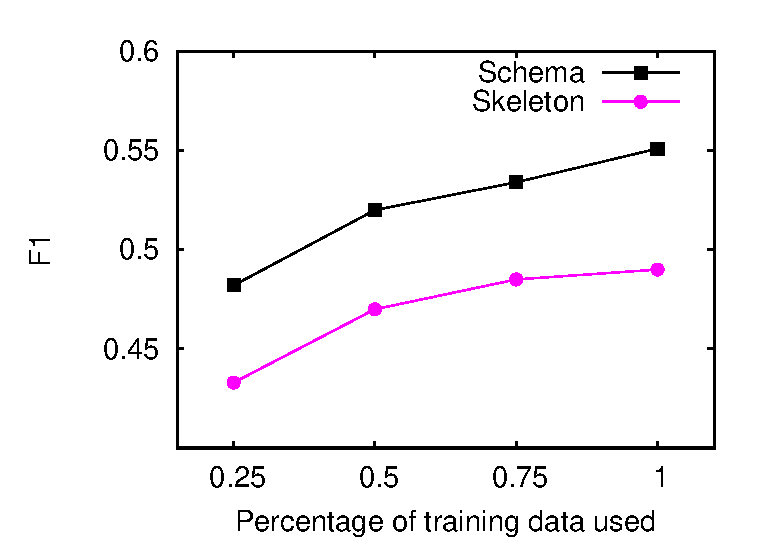
\epsfig{file=trend.eps, width=0.65\columnwidth}
\centering
\caption{F1 result vs. amount of training data.}
\label{fig:trend}
\end{figure}

%We split the complex relation dataset into 41 training and
%20 testing relations. Only training relations are used to learn our model.
%For each test relation, we split all instances into 80\% observable and
%20\% hidden parts to be predicted.
%We generate candidate schemas on the observable part
%(without computing silver labels)
%and calculate schema probability distribution from learned feature weights.
%Then our system scores each hidden entity pair by summing the probability
%of all schemas that cover this pair.
%As a prediction task, negative entity pairs are added in the hidden part.
%Based on annotated schemas for each relation,
%we automatically sample negative data from those entity pairs
%which are not covered by the schema but covered by its skeleton.
%In addition, our system retained 20\% data in the observable part
%as validation set, which is used to tune a cut-off score for
%each test relation.

We compare our approach with state-of-the-art KBC system by
Gardner et al. \shortcite{gardner2015efficient}.
We perform its best setting SFE-AnyRel (subgraph
+ wildcard paths) and SFE-OneSided (subgraph + one-side paths),
which is most similar to our model.
Both settings need negative relation instances at their training step, while we don't.
%therefore we follow their algorithm, generating negative pairs
%by close world assumption.
%Besides, we need negative pairs for tuning in validation set,
%and we also sample negative pairs by close world assumption.
%As a baseline approach, we run our system under skeleton mode,
%that is, only keeping skeletons in the step of candidate schema generation.
Due to memory limit on their system, we construct a subset of the Freebase, named as $FB^-$.
It consists of top 3,000,000 popular entities as well as necessary mediators connecting those entities.
%We first pick the top 3,000,000 popular entities from Freebase by its frequency among all different triples,
%and keep all intermediate entities that connect at least 2 popular entities.
All direct predicates between entities and all IsA relations are retained in the subset.
\tabref{tab:fb-size} shows the scale comparison between $FB^-$ and the original Freebase.
We believe the subset carries enough meaningful facts from Freebase since all top entities are kept.
%Since we have kept all top entities, we believe that $FB^-$ carries enough useful facts from Freebase 
%(though it covered only 11.9\% entities and 20.7\% facts of the original FB).
As shown in the bottom part of \tabref{tab:kbc-complex}, our schema-based approach reaches the best F1 score at 0.547.
Compared with SFE-OneSided, our approach improved the result by 12.8\%.
Due to constraints imposed to structural representations, schema and SFE-OneSided approach 
show a conservative prediction but controls a nice balance on precision and recall,
while SFE-AnyRel works aggressively and failed to make a good trade-off.

%\begin{table}[ht]
%\small
%	\centering
%	\caption{Results of KBC task on 61 complex relations.}
%	\begin{tabular}{|l|c|c|c|}
%	%	%\toprule
%		\hline
%		Approach				 & Precision & Recall & F1 \\
%        \hline
%        \hline
%        Schema					 & \textbf{0.571} & 0.468 & \textbf{0.514} \\
%        \hline
%        Skeleton				 & 0.470 & 0.488 & 0.479 \\
%		\hline
%        SFE-AnyRel				 & 0.391 & \textbf{0.538} & 0.453 \\
%		\hline
%		SFE-OneSide				 & 0.457 & 0.442 & 0.450 \\
%		\hline
%	\end{tabular}%
%	\label{tab:kbc-complex-with-sfe}%
%\end{table}



\subsection{KBC Evaluation on Ordinary Relations}
Now we compare our system with previous work on an ordinary relation dataset, which
contains 100 relations randomly sampled from top PATTY relations.
Following the previous setting, we split relations instances into 
80\% training and 20\% testing, and we also generate negative instances by close world assumption.
%While not all relations can be annotated with a schema (not skeleton) in
%this dataset, thus, negative relation instances in test set are generated
%by close world assumption.
%just running full version is okay, if there's no time.
Evaluation results are shown in \tabref{tab:kbc-ordinary}.
Compared with results on complex relations, we make two discoveries.
First, schema based approach only maintains a smaller edge over other methods,
because skeleton representation is often sufficient for ordinary, simple relations.
Second, for all approaches, F1 scores on ordinary dataset are generally
lower than those for the complex dataset.
The main reason is that, PATTY contains a lot of common but trivial relations
like \textit{``(PER) talked to (PER)''},
\textit{``(PER) spent years in (LOC)''},
though they are frequently mentioned in web corpus,
a typical KB doesn't have proper predicates to represent such relations.

%\begin{table}[ht]
%%\small
%	\centering
%	\caption{Results of KBC task on 100 ordinary relations.}
%	\begin{tabular}{|l|c|c|c|c|}
%		%\toprule
%        \hline
%		Approach				 & Dataset & Precision & Recall & F1 \\
%        \hline
%        \hline
%        Schema					 & $FB$ & 0.289 & 0.436 & \textbf{0.347} \\
%        \hline
%        Skeleton				 & $FB$ & 0.274 & 0.439 & 0.338 \\
%		\hline
%		Schema					 & $FB_{sub}$ & 0.xxx & 0.xxx & 0.xxx \\
%		\hline
%        SFE-AnyRel				 & $FB_{sub}$ & 0.231 & \textbf{0.536} & 0.323 \\
%		\hline
%		SFE-OneSide				 & $FB_{sub}$ & \textbf{0.351} & 0.280 & 0.312 \\
%		\hline
%	\end{tabular}%
%	\label{tab:kbc-ordinary}%
%\end{table}


\begin{table}[ht]
	\small
	\centering
	\caption{KBC results on 100 randomly sampled relations.}
	\begin{tabular}{|c||c|c|c|c|}
		%\toprule
		\hline
		Dataset					& Approach	& Precision & Recall & F1 \\
        \hline
		\multirow{2}{*}{$FB$}	& Schema	& \textbf{0.388} & \textbf{0.485} & \textbf{0.431} \\
		\cline{2-5}
        						& Skeleton	& 0.381 & 0.478 & 0.424 \\
		\hline
		\multirow{4}{*}{$FB^-$} & Schema		& 0.371 & 0.491 & 0.423 \\
		\cline{2-5}
								& Skeleton		& 0.380	& 0.490	& \textbf{0.428}	\\
		\cline{2-5}
								& SFE-AnyRel	& 0.306	& \textbf{0.562} & 0.396	\\
		\cline{2-5}
								& SFE-OneSided	& \textbf{0.448}	& 0.351 & 0.394	\\
		\hline
	\end{tabular}
	\label{tab:kbc-ordinary}
\end{table}


\subsection{Result Analysis}
Finally, we analyze the performance of our learned schemas in more detail.
\begin{figure*}[th]
 \epsfig{file=case_crop.eps, width=1.05\columnwidth, angle=270}
\centering
\caption{An example fragment of schema paraphrasing results.
We list top-3 schemas along with probabilities for each relation.
Circle node indicates entities or variables, the two black circles represents
$x_{subj}$ and $x_{obj}$ respectively. Square node represents a type, and
round square node represents a mediator (auxiliary node to organize an n-ary fact).}
\label{fig:relation-example}
\end{figure*}
\figref{fig:relation-example} shows the paraphrasing results of example relations.
%Show a case-by-case P/R/F1/RR?
The results of top-ranked schemas show us that our paraphrasing system
is able to produce concrete and precise structural representations,
but in several cases, the system failed to paraphrase the relation into
correct semantics. We have analyzed relations in the above experiments and
find several main causes of error.

1. Relation instances extracted by Open IE system could be incorrect.
PATTY extracts relation instances by mining the dependency path in a sentence,
which may lead to wrong arguments.
For example, given the relation \textit{``served as''}, PATTY extracted
an incorrect entity pair (William Dennison Jr., Ohio) from the sentence
\textit{``Dennison served as the 24th Governor of Ohio and as U.S. Postmaster General ...''},
while the correct object should be ``Governor of Ohio''.

2. PATTY relation synset mixed semantic different but lexical similar
relation patterns, bringing noisy entity pairs in the relation.
For example, in PATTY's \textit{``'s wife''} relation synset, we found a small list of instances
where the object is actually husband.
These instances represents the exact opposite semantics,
due to the pattern \textit{``the wife of''} is mixed in the synset.
Though our system is able to filter out noisy instances, the learned schema
distribution would be affected if the percentage of noisy data goes larger.

3. Knowledge base lacks of necessary information for paraphrasing certain relations.
As mentioned before, Freebase doesn't hold knowledge about trivial relations.
Even paraphrasing non-trivial relations, required predicates could be missing in Freebase.
Given the relation \textit{``(singer) is performed in (LOC)''}, FB contains			% synset 0246
neither \textit{place\_visited} nor \textit{hold\_concerts\_in} predicate, therefore
our system is not able to summarize into a precise representation.

4. Sometimes a meaningful schema is filtered due to limits in candidate searching step.
In relation \textit{``(actor) starring with (actor)''}, the length of the most suitable skeleton
\footnote{The skeleton is $actor \rightarrow med. \rightarrow film \rightarrow med. \rightarrow actor$.}
is 4, hence the system failed to discover it under restriction $\tau$ = 3.


%\subsection{QA Evaluation on Complex Relations}
%We perform a question answering experiment over complex relations.
%This task is known to automatically answer human raised questions represented by purely string.
%In order to justify the usefulness of complex schemas, we manually pick 120 test questions from WebQuestions \cite{berant2013semantic}.
%Each question includes one of the 20 complex relations that
%we tested in the earlier KBC experiment.
%We use learned schemas for querying and voting answers,
%resulting in a ranked answer list.
%We compare our results with the work of
%Yao et al. \shortcite{yao2014information}
%as well as Berant and Liang \shortcite{berant2014semantic}.
%We provide the correct subject entity in the question to each system,
%and link the question to the corresponding PATTY relation,
%since entity resolution and relation mapping steps are not our focus.
%
%We control the number of returned answers from each question as $k$,
%and evaluate F1 score over different $k$ values.
%The detailed results are shown in \tabref{tab:qa-f1}, which
%shows that our approach using complex schema outperforms by
%large margins in both macro and micro F1.
%By inferring schemas for those questions with complex relations,
%our method essentially brings in fresh semantic information from Open IE,
%which is not available to other competing methods.
%
%\begin{table}[ht]
%\small
%	\centering
%	\caption{F1 of QA task on 120 complex questions}
%	\begin{tabular}{|l|c|c|c|}
%		%\toprule
%        \hline
%        \multicolumn{4}{|c|}{Macro F1} \\
%        \hline
%						 & k=1 & k=2 & k=3 \\
%        \hline
%        Schema			 & \textbf{0.482} & \textbf{0.545} & \textbf{0.563} \\
%        \hline
%        Berant & 0.436 & 0.495 & 0.453 \\
%		\hline
%        Yao				 & 0.297 & 0.368  & 0.394 \\
%		\hline
%		\multicolumn{4}{|c|}{Micro F1} \\
%		\hline
%						 & k=1 & k=2 & k=3 \\
%        \hline
%        Schema			 & \textbf{0.444} & \textbf{0.511} & \textbf{0.523} \\
%        \hline
%        Berant & 0.362 & 0.432 & 0.492 \\
%		\hline
%        Yao				 & 0.217 & 0.304  & 0.352 \\
%		\hline
%	\end{tabular}%
%	\label{tab:qa-f1}%
%\end{table}
%
%
%\subsection{Relation Similarity Task Evaluation}
%In this experiment, we evaluate the framework's ability to
%calculate the similarity between two natural language relations.
%The task takes as input a pair of PATTY relations, for example
%``{\em PER} be professor at {\em LOC}'' and ``{\em PER}
%teaches in {\em LOC}'', and predicts whether these
%two relations are similar or not.
%To automatically generate test pairs, we leverage
%PPDB \cite{ganitkevitch2013ppdb} as an external resource of gold paraphrases,
%which contain pairs like ``is professor'' and ``teaches''.
%We label a relation pair as positive if it can be linked
%to a phrase pair in PPDB by fuzzy string match,
%and generate negative pairs by random combining.
%The experiment dataset contains 45 positive and 90 negative relation pairs,
%with 77 distinct relations in total.
%
%We used the model trained on 41 complex relations for this task.
%For each relation pair, we calculate both cosine and
%generalized Jaccard similarity
%between schema probability distribution on those relations.
%We compare our result with a baseline word2vec model \cite{mikolov2013word2vec},
%where the vector representation of a relation is computed
%by averaging embedding vectors over all its surface words,
%and use cosine similarity as the measurement.
%
%\begin{figure}[th]
%\centering
%\epsfig{file=pr.eps,width=\columnwidth}
%\caption{PR curves for relation similarity.}
%\label{fig:pr}
%\end{figure}
%
%\figref{fig:pr} shows the precision-recall curves from the three
%approaches. One can see that schema representation is very competitive
%against the popular word embedding representation in the similarity
%task. Furthermore, \tabref{tab:rel-sim} gives the AUC (area under curve)
%of the three curves and indicates that the two variants using schemas
%perform even slightly
%better than word2vec.
%This suggests that KB schema distribution is a viable representation
%for modeling natural language relations.
%
%\begin{table}[ht]
%\small
%	\centering
%	\caption{Results on relation similarity task.}
%	\begin{tabular}{|l|c|}
%		%\toprule
%        \hline
%		Approach				 & AUC \\
%        \hline
%        \hline
%        Schema + Cosine			 & {\bf 0.709} \\
%        \hline
%        Schema + Jaccard		 & 0.706 \\
%		\hline
%        word2vec + Cosine		 & 0.705 \\
%		\hline
%	\end{tabular}%
%	\label{tab:rel-sim}%
%\end{table}

%\begin{table}[ht]
%	\centering
%	\caption{F1 of QA task on 120 complex questions}
%	\begin{tabular}{|l|c|c|c|}
%		%\toprule
%        \hline
%        \multicolumn{4}{|c|}{Macro F1} \\
%        \hline
%						 & k=1 & k=2 & k=3 \\
%        \hline
%        Schema					 & 0.448 & 0.545 & 0.574 \\
%        \hline
%        Skeleton				 & 0.316 & 0.457 & 0.374 \\
%		\hline
%        SFE-AnyRel				 & 0.260 & \textbf{0.513} & 0.345 \\
%		\hline
%		\multicolumn{4}{|c|}{Micro F1} \\
%		\hline
%						 & k=1 & k=2 & k=3 \\
%        \hline
%        Berant					 & 0.436 & 0.495 & 0.453 & 0.362 & 0.432 & 0.492 \\
%		\hline
%        Yao						 & 0.297 & 0.368 & 0.394 & 0.217 & 0.304  & 0.352 \\
%		\hline
%	\end{tabular}%
%	\label{tab:qa-f1}%
%\end{table}



%1. alternative of MDL, check difference on principles
%2. ablation test, DFS/ without DFS
%3. state-of-the-art, find new papers
%4. VELVET 2012 implementation
%5. entity linking (self, others)
%6. make bfs faster. robustness even in noisy situation
%(optional) 6. down-streaming application (QA?)
